%%% template.annotated.tex
%%%
%%% This LaTeX source document can be used as the basis for your technical
%%% paper or abstract. Unlike ``template.tex,'' this version of the source
%%% document contains documentation of each of the commands and definitions
%%% that should be used in the preparation of your formatted document.
%%% 
%%% The parameter given to the ``acmsiggraph'' LaTeX class in the 
%%% ``\documentclass'' command controls several features of the formatted 
%%% output: the presence or absence of hyperlinked icons just prior to the 
%%% first section of the paper, the amount of space left clear for the ACM
%%% copyright notice, the presence or absence of line numbers and submission
%%% ID, and the presence or absence of an appropriate ``preprint'' notice.
%%% 
%%% If you are preparing a paper for presentation in the Technical Papers
%%% program at one of our two annual flagship conferences, held in North 
%%% America (SIGGRAPH) or Asia (SIGGRAPH Asia), you should use ``tog''
%%% as the parameter.
%%%
%%% If you are preparing a paper for presentation at one of our sponsored
%%% events, including SIGGRAPH and SIGGRAPH Asia, but not in those events' 
%%% Technical Papers program, or a one- to four-page abstract, you should 
%%% use ``conference'' as the parameter.
%%% (Technical Briefs and Game Papers presented at our annual flagship 
%%% events fall into this category, as do papers accepted to other SIGGRAPH-
%%% sponsored events, such as I3D or ETRA or VRCAI, as do the one-page 
%%% abstracts which serve as the primary documentation for many of our 
%%% annual conference programs, including Posters, Talks, and Emerging 
%%% Technologies.)
%%%
%%% If you are preparing a version of your content for review, you should
%%% use ``review'' as the parameter. Line numbers will be added to your 
%%% paper, and the submission ID value will be printed across the top of 
%%% each page of your paper. (Use the submission ID as the parameter to the
%%% ``TOGonlineID'' command, below.)
%%%
%%% If you are preparing a preprint of your content, you should use
%%% ``preprint'' as the parameter. This is primarily for annual conference
%%% papers; a header reading ``To appear in ACM TOG X(Y)'' will appear on
%%% each page of the formatted output (where X is the volume and Y is the 
%%% number of the issue in which it will be published).

\documentclass[tog]{acmsiggraph}

%%% Definitions and commands that begin with ``\TOG'' are meant to be used
%%% in the preparation of papers to be presented in the Technical Papers
%%% program at one of our annual flagship events - SIGGRAPH and SIGGRAPH 
%%% Asia. You can safely ignore these definitions and commands if your 
%%% content is to be presented in some other venue.

%%% ``\TOGonlineid'' should be filled with the online ID value you received
%%% when you submitted your technical paper. It will be printed out if you 
%%% prepare a ``review'' version of your paper.

\TOGonlineid{45678}

%%% Should your technical paper be accepted, you will be given three pieces
%%% of information: the volume and number of the issue of the ACM Transactions
%%% on Graphics journal in which your paper will be published, and the 
%%% ``article DOI'' value, which is unique to your paper and provides the 
%%% link to your paper's page in the ACM Digital Library. Fill in the 
%%% ``\TOGvolume,'' ``\TOGnumber,'' and ``\TOGarticleDOI'' definitions with
%%% the three pieces of information you receive.

\TOGvolume{0}
\TOGnumber{0}
\TOGarticleDOI{1111111.2222222}

%%% By default, your technical paper will contain hyperlinked icons which 
%%% point to your paper's article page in the ACM Digital Library, and to 
%%% the paper itself in the ACM Digital Library. You may wish to add one 
%%% or more links to your own resources. If any of the following four 
%%% definitions have URLs in them, an appropriate hyperlinked icon will be
%%% added to the list. 

\TOGprojectURL{}
\TOGvideoURL{}
\TOGdataURL{}
\TOGcodeURL{}

%%% Define the title of your paper here. Use capital letters as appropriate.
%%% Setting the entire title in upper-case letters is not correct, nor is 
%%% capitalizing only the first letter of the title.

\title{Fracture Simulation via Convex Decomposition in Two Dimensions}

%%% Define the author list in the ``\author'' command. The ``\thanks'' 
%%% field can be used to define an e-mail address for the author.
%%% The ``\pdfauthor'' field should contain a comma-separated list of the
%%% authors of the paper, and is used, along with the title and keyword
%%% data, for PDF metadata. (To see this metadata, open the PDF in Adobe 
%%% Reader and select ``File > Properties > Description.''

\author{Ari Karo, Chris
  Yu\thanks{e-mail:\{aak82,cy284\}@cornell.edu}\\Cornell University}
\pdfauthor{Stanford Bunny}

%%% User-defined keywords.

\keywords{cs5643, final project, proposal, fracture simulation}

%%% End of the document preamble, start of the document.

\begin{document}

%%% A ``teaser'' image appears below the title and affiliation and above
%%% the two-column body of the paper. This is optional, but if you wish
%%% to include such an image, the commented-out code, below, can be used
%%% as an example. Please note that the inclusion of a ``teaser'' image
%%% may move the copyright space to the bottom of the right-hand column
%%% on the first page of your formatted output. This is acceptable.

 \teaser{
   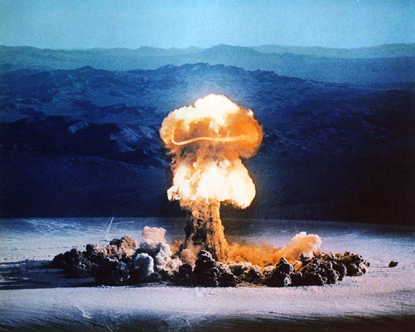
\includegraphics[height=1.5in]{images/explode.jpg}
   \caption{An example of a scenario that may call for fracturing objects.}
}

%%% The ``\maketitle'' command uses the author and title information 
%%% defined above, and prepares the formatted title.

\maketitle

%%% The ``abstract'' environment should contain the abstract for your
%%% content -- one to several paragraphs which describe the work.

\begin{abstract}

Here, we discuss our implementation of dynamic fracture simulations,
as detailed in \cite{Mul13}. The method described is an improvement on
previous methods for fracture simulations, which typically involve
using pre-fractured models and replacing objects with these fragments
at runtime. These older methods have the disadvantage that fracture
patterns generally do not match the impact location. The newer method
uses volumetric approximate convex decompositions (VACDs), whereby
pre-defined fracture patterns are applied to the pieces of geometry,
and the geometry is subsequently split into a non-overlapping convex
cover of itself. We present our implementation of a two-dimensional
analogue of the algorithms given, and discuss our findings and
results.

\end{abstract}

%%% The ``CRCatlist'' environment defines one or more ACM ``Computing Review''
%%% (or ``CR'') categories, used for indexing your work. For more information
%%% on CR categories, please see http://www.acm.org/class/1998.

\begin{CRcatlist}
  \CRcat{5643}{Computer Graphics}{Physically Based Animation}{Fracturing}
\end{CRcatlist}

%%% The ``\keywordlist'' prints out the user-defined keywords.

\keywordlist

%%% If you are preparing a paper to be presented in the Technical Papers
%%% program at one of our annual flagship events (and, therefore, using 
%%% the ``tog'' parameter to the ``\documentclass'' command), the 
%%% ``\TOGlinkslist'' command prints out the list of hyperlinked icons.
%%% If you are using any other parameter to the ``\documentclass'' command
%%% this command does absolutely nothing.

%\TOGlinkslist

%%% The ``\copyrightspace'' command will leave clear an amount of space
%%% at the bottom of the left-hand column on the first page of your paper,
%%% according to the parameter used in the ``\documentclass'' command.

\copyrightspace

%%% The first section of your paper. 

\section{Introduction}

Simulations of fracturing objects are becoming increasingly applicable
and desirable in media such as movies and games, where, depending on
the genre, scenes of massive and wanton destruction may be
commonplace. Particularly in the context of video games, the prospect
of every rigid object being indestructible may be perceived as
implausible by an observer. While pre-fracturing is an option for
interactive simulations, this requires additional work for every
breakable asset, and prevents the pattern of fracture from depending
on the point of impact. There are also various other drawbacks, such
as pieces of objects being unable to break further without
preemptively preparing multiple levels of pre-fracturing.

A dynamic fracture simulation could potentially save time in producing
these assets, in addition to providing additional realism by allowing
objects to fracture in different ways, depending on the direction and
location of impact. In \cite{Mul13}, M\"uller et al. present a new
method for such dynamic fractures, which simultaneously preserves
interactive speeds.

\section{Related Work}

The primary paper we will be focusing on is M\"uller et
al. \cite{Mul13} where the methods and algorithms for dynamic fracture
simulation are presented. Before this paper, various other methods for
fracture simulation had been described, dating back as early as
Terzopoulos et al. \cite{Ter88} and Norton et al. \cite{Nor91}, the
latter making use of a mass-spring model. O'Brien et al. \cite{Obr99}
presented a method that used continuum mechanics to compute internal
stresses and fracture directions.

Parker et al. \cite{Par09} proposed a method for fracture simulation
that used a relatively coarse tetrahedral mesh, where objects can
fracture only along the bounaries of the tetrahedra; in order to hide
the coarseness of the mesh, they also introduce ``splinters''
associated with each element. This method is primarily targeted at
computer games, as it runs at interactive speeds.

Pre-fracturing objects is a commonly-used approach in movies and
games, as mentioned, and a wide array of methods for breaking up
objects has been proposed. A few of the many techniques include manual
cutting by artists, image guidance \cite{Mou05}, Voronoi fracturing of
surfaces \cite{Rag02}, and tetrahedralization \cite{Par09}.

\section{Technical Description}

The method described only works with meshes that satisfy the following
three properties: (1) the meshes are composed of convex pieces, (2)
the pieces do not overlap, and (3) any two pieces are physically
connected if and only if the first piece has at least one face that
partially or fully overlaps one face of the second piece, and the two
faces are coplanar with opposite normals. A mesh satisfying this is
called a compound. Note that meshes created by volumetric approximate
convex decomposition satisfy this property by default; the exact
algorithm for performing the VACD is given in the paper.

The method uses fracture patterns, which are partitions of the entire
space into convex pieces. Once fracturing is called for, the following
steps are performed. The fracture pattern is first translated to align
with the impact location. We then compute all intersections of all
cells of the fracture pattern with all convex pieces of the
object. Next, in order to save computation time, we find all pieces
that are completely covered with newly created convexes, and replace
these all with a single convex with the same shape. All convexes
within the same cell are then combined to form a new
compound. Finally, we check for disconnected ``islands'' of convexes
that have been grouped into the same mesh, and turn them into separate
compounds.

\section{Implementation Details}

Due to the time constraints on the project, we decided against
implementing the full algorithm in three dimensions, and instead chose
to implement an adapted algorithm for two dimensions. Our system
performs the same general computations, but specialized for two
dimensions rather than three.

Because implementing a rigid-body system in itself no simple task, in
order to allow ourselves to focus on the fracture simulation, we
decided to use an existing physics engine to handle basic rigid body
mechanics and collisions. The system we decided upon was dyn4j
(http://www.dyn4j.org/), a simple 2d rigid body library.

\subsection{Convex Geometry}

We implemented some functions related to convex geometry. The first
was an algorithm for generating the convex hull of a set of points. We
implemented the monotone chain algorithm \cite{Andrew79}, which
essentially functions by constructing the top and bottom chains of the
points and then combining the two chains, running in $O(n \log n)$
time. We then also implemented an algorithm for taking the
intersection of two convex polygons. The algorithm is not very
advanced, in that it simply chooses the vertices of each polygon that
are inside the other, adds the intersection points of any edges of the
polygons, and then creates the convex hull of that set of points,
running in $O(n^2)$. However, because the expected number of vertices
per polygon is quite small (in many cases, no more than 10), this does
not constitute a significant performance hit. Over the course of
implementing these algorithms, we also implemented various other
utility functions, including distance functions between points, lines,
and polygons.

We implemented a simple class to wrap a convex polygon, which
encapsulates details such as body space to world space
transformations, and creation of convex polygons from point clouds
using the aforementioned algorithm. In order to extend support for
non-convex polygons, we created another class for a ``welded''
polygon, which is a set of convex polygons welded together. Using this
welding, polygons of any shape can be created, provided they do not
have holes. At this point, in order to allow the user to input a
non-convex polygon, we need to decompose the non-convex polygon into a
set of convex polygons. M\"uller et al. use a volumetric approximate
convex decomposition (VACD) algorithm that is specialized for
3D. However, in 2D, there are simpler solutions than the one detailed
in the paper; we opted to use an ear clipping algorithm that was
already provided by dyn4j.

M\"uller et al. use fracture maps, partitions of all of space into
convex regions, in order to perform their fracturing. We implemented a
fairly na\"ive Voronoi diagram algorithm in order to create fracture
maps. Our algorithm computes the cell of each point by beginning with
the $1 \times 1$ square as the convex cell, and then, for each other
point, computing the perpendicular bisector with that point and
dividing the current convex cell across that line. Dividing the cell
takes $O(n)$ time in the number of vertices; this is done for the $n$
other points in the diagram, and the algorithm generates $n$ cells, so
the algorithm runs in $O(n^3)$. However, the Voronoi diagrams we will
be using will in all likelihood have fewer than 100 points, and the
diagram only needs to be computed when a new fracture map is input, so
the overall effect on performance is negligible. The fracture maps are
stored as sets of convex polygons that partition the unit square.

\subsection{Overview of Fracture Algorithm}

Fractures can be triggered by either direct user input or other means
(to be discussed later). When a convex polygon is fractured, we make
the assumption that the point of impact lies inside the polygon
itself, an assumption that holds in all circumstances of our system.
The fracture algorithm then proceeds as follows.

\begin{enumerate}

\item The current fracture pattern is translated so that it is
  centered at the point of impact.

\item In the case of a welded polygon, the bounding box of all
  convexes within a predefined impact radius of the point is taken,
  and the fracture pattern is scaled so that it contains all of these
  nearby convexes, while remaining centered at the point of impact.
  In the case of a simple convex, the bounding box of the convex is
  used.

\item All convexes within the impact radius are intersected with the
  cells of the fracture map, resulting in a set of convex pieces
  occupying the same space.

\item Any of the original convexes that were outside of the impact
  radius, as well as any newly-created convexes that are outside of
  the radius, are all grouped together.

\item Island detection is performed on the distant polygons, which
  splits any disjoint groups of polygons into separate bodies.

\item A predefined impulse is applied outward from the impact point to
  all newly created bodies, causing the fractured pieces to move
  apart.

\item The linear velocity of the fractured convex is transferred to
  all of the new convexes.

\end{enumerate}

Our island detection algorithm iteratively removes islands from the
set of polygons being considered. It chooses one polygon and performs
a breadth-first search outward, adding polygons to the frontier if
they are in contact with the current polygon. Once no more polygons
can be explored, a connected component has been found, and the
explored polygons are merged into a new welded polygon and removed
from consideration. The algorithm then repeats until the set of
polygons is empty.

\subsection{User Interactivity}

We have implemented multiple features to allow users to interact more
directly with the simulation. Users are able to click and drag
existing convexes on the screen to move them around. This is done by
way of a spring constraint between the object and the current mouse
position. Users can also create convex polygons by inputting a set of
points, whereupon the convex hull algorithm is called to create a new
polygon. Users can create a non-convex polygon by inputting a chain of
points that comprises the boundary of the polygon; convex
decomposition is then run to create a welded polygon with the same
shape. Note that the polygon must be simple, meaning that edges cannot
cross each other. There is no way to input polygons with holes.

We enable users to define their own fracture patterns. This is done by
first presenting the user with a blank canvas, and allowing them to
input multiple control points. The resulting fracture map is the
Voronoi diagram of the given control points. Users can also save and
load fracture maps to and from the disk, and cycle between multiple
maps that they have created.

Users have two ways to trigger fractures. The first way is by clicking
on convexes directly; in this case, the resulting point of impact is
wherever the user clicked, and the piece is fractured accordingly. The
second way is by firing projectiles. Upon selecting this option, the
user is able to specify the location in the space from which the
projectiles should originate. Then, they are able to click on a
location toward which the projectiles will be launched. Upon clicking,
a projectile in the shape of a thin triangle is emitted at high speed
from the origin point in the given direction. The projectile will
fracture whatever polygons it comes in contact with; it is removed
when it either leaves the bounds of the box, or fractures a set number
of polygons. Note that projectiles have infinite mass, meaning that
they do not collide with other objects (including other projectiles),
and cannot be deflected from their paths.

\section{Results and Discussion}

We found that the plausibility of this fracture simulation algorithm
depends heavily on the fracture pattern being used. If the fracture
pattern seems unnatural, in that it may have too many regular
geometric shapes or other artificial-seeming features, then the
resulting fractures do not seem believable. If, however, the fracture
pattern seems more natural and chaotic, then the resulting fractures
do seem sufficiently plausible. From our experiments, ``good'' fracture
patterns tend to have smaller pieces closer to the center of the
pattern, and the pieces tend to spread radially outward. One reference
for such a pattern might be the pattern on a sheet of glass when it is
strongly impacted at a point. When such a pattern is used, the
resulting fracture creates smaller pieces closer to the point of
impact, and farther away, the cracks are more widely spread apart, as
might be expected.

The addition of the impulse that separates the fractured pieces also
aids with plausibility. Without this impulse, the pieces will tend to
remain locked in the same shape, due to the fact that the fracture
pattern fits tightly together with no gaps. With the impulse, the
pieces separate visibly, giving the impression of a breaking
object. This especially applies to the projectile mode of causing
fractures, where there is an expectations for the pieces to be
launched at considerable speed due to the impact.

In terms of performance, the runtime of the fracturing routines
themselves is quite fast; several fractures can be processed at the
same time within the simulation without noticeable slowdown. In fact,
the majority of the slowdown comes from the need to perform rigid body
computations on the resulting fractured pieces, which is separate from
the fracture code. In particular, much of the slowdown is due to very
small pieces that are created from fractures. Despite the
non-optimality of some of the algorithms we are using for geometry and
fracturing, the numbers involved are small enough that the running
time is dwarfed by the running time of the rigid body simulation
itself. A similar fact is true for the convex hull and Voronoi
algorithms; in this case, because the input size is determined by the
user, and because the algorithms are only run when the user requests
them, the overall time spent running these algorithms is quite low
compared to the rest of the program.

Fracturing large convex objects can result in some very large pieces
splitting off from each other, due to the fact that the fracture
pattern must be scaled to cover the entire object. In this case, one
might expect instead only some local fracturing, instead of the
splitting of the entire object. This can be alleviated somewhat by
simply generating more detailed fracture patterns; a more robust
solution might be to extend the existing Voronoi diagram to cover the
expanded space rather than just scaling the entire diagram, though we
have not implemented this. Welded polygons do not share this same
problem, because the diagram need only be scaled to cover the pieces
within the radius, which typically do not comprise the entire object.

In fact, the fracture pattern approach is fairly easily extendable;
some modifications that we might consider would be to select different
fracture patterns (perhaps randomly) according to the magnitude of the
impact force, or to allow additional transformations to fracture
patterns such as rotations. Additional directions for exploration are
also mentioned in the paper; these include causing objects to fracture
under their own weight, and modeling the fact that objects do not
necessarily only fracture at one point. While these would require some
additional computations (in particular, stress analysis for the
former), the fracturing process itself could still be handled by
fracture patterns.

While the method is not completely physically accurate in that it does
not compute the fracture lines according to internal stresses of the
objects, that is not the purpose of this method. Instead, this method
provides plausible fracturing, with the advantage that the fracturing
process is quite fast, and with some optimization, it can be fast
enough to run at interactive speeds. With some controlling of the
number of tiny pieces that are created, and further tuning of the
parameters, our project could easily be the start of an interactive
application or game involving physics and fracturable objects.

\bibliographystyle{acmsiggraph}
\bibliography{template}

\end{document}
